

%%% Models and Results %%%
\section{Models and Results}
Para la estimación de los modelos de predicción de pobreza se consideraron diversos algoritmos orientados a problemas de clasificación binaria. Estos pueden agruparse en dos grupos: modelos lineales y modelos basados en árboles. En el primer grupo se incluyen la Regresión Logística (Logit) y su versión penalizada mediante Elastic Net (Logit Elastic Net). La elección de estos modelos responde a la necesidad de aproximar una frontera de decisión lineal, siendo la Regresión Logística un punto de partida fundamental en tareas de clasificación supervisada. La regularización vía Elastic Net introduce penalizaciones L1 y L2 sobre los coeficientes, con el propósito de reducir la varianza del estimador y, en consecuencia, mejorar su capacidad de generalización.

Complementariamente, se exploraron modelos basados en Árboles de Clasificación y Regresión (CART), tanto de manera individual como a través de métodos de ensamblaje. Aunque los árboles simples suelen presentar alta varianza, su combinación en algoritmos de ensamble como Random Forest y XGBoost permite obtener modelos robustos y de excelente desempeño empírico, al capturar interacciones y no linealidades entre los predictores. Esta propiedad resulta particularmente relevante en contextos donde las relaciones entre las variables explicativas y el resultado son complejas y difíciles de especificar de forma paramétrica. Todos los modelos fueron entrenados sobre la misma base de entrenamiento y evaluados sobre la misma base de prueba. 


Es importante precisar las métricas utilizadas en la evaluación del modelo binario (Sí, No). El desempeño se mide a partir de la matriz de confusión, en la cual los verdaderos positivos (\textbf{TP}) corresponden a los hogares correctamente clasificados como pobres, los falsos positivos (\textbf{FP}) a los que fueron identificados como pobres sin serlo, los verdaderos negativos (\textbf{TN}) a los correctamente clasificados como no pobres y los falsos negativos (\textbf{FN}) a los que, siendo pobres, el modelo clasificó como no pobres . Estos cuatro elementos conforman la matriz de confusión presentada en la Tabla \ref{tab:confusion_ejemplo}.

\begin{table}[ht]
\centering
\caption{Matriz de confusión}
\label{tab:confusion_ejemplo}
\begin{tabular}{lccc}
\toprule
 & \multicolumn{3}{c}{\textbf{Verdadero}} \\
\cmidrule(lr){2-4}
 &  & \textbf{Sí} & \textbf{No} \\
\midrule
\multirow{\textbf{Predicho}} 
 & \textbf{Sí} & TP & FP \\
 & \textbf{No} & FN & TN \\
\bottomrule
\end{tabular}
\end{table}

De estos cuatro componentes se derivan tres métricas principales que permiten evaluar el desempeño del modelo: la precisión (\textbf{Precision} \ref{eq:metrics}), que mide la proporción de hogares correctamente identificados como pobres entre todos los clasificados como tales; la sensibilidad (\textbf{Recall} \ref{eq:metrics}), que refleja la capacidad del modelo para identificar correctamente a los hogares pobres; y el \textbf{F1} \ref{eq:metrics}, que corresponde a la media geométrica entre el precision y recall. Estas métricas se eligen debido al desbalance presente en la predicción de pobreza monetaria, y se mantienen en inglés por coherencia con la literatura y los reportes de resultados del modelo.

\begin{equation}
\text{Precision} = \frac{TP}{TP + FP}, \quad
\text{Recall} = \frac{TP}{TP + FN}, \quad
F1 = 2 \times \frac{\text{Precision} \times \text{Recall}}{\text{Precision} + \text{Recall}}
\label{eq:metrics}
\end{equation}

\subsection{Selección de  hiperparámetros y modelos}

La selección de hiperparámetros se llevó a cabo mediante validación cruzada estratificada en cinco particiones, buscando equilibrar la exhaustividad en la exploración del espacio de parámetros y la viabilidad computacional del procedimiento.

\begin{table}[!h]
\centering
\small
\caption{Resultados de la validación cruzada en la selección de modelos}
\label{tab:cross_validation}
\begin{tabular}{p{2.8cm} p{5cm} p{4cm} ccc}
\toprule
\textbf{Algoritmo} & \textbf{Rangos de búsqueda} & \textbf{Mejor modelo} & \textbf{F1} & \textbf{Recall} & \textbf{Precision} \\
\midrule
\shortstack[l]{Logit} & --- & --- & 0.654 & 0.595 & 0.726 \\
\addlinespace[6pt]

\shortstack[l]{Logit\\Elastic Net} & 
\shortstack[l]{alpha [0–1]\\lambda [0.001–1000]} &
\shortstack[l]{alpha = 0.5\\lambda = 0.001} &
0.647 & 0.585 & 0.725 \\
\addlinespace[6pt]

\shortstack[l]{CART} & 
cp [2e-04–0.0628] &
cp = 2e-04 &
0.651 & 0.602 & 0.710 \\
\addlinespace[6pt]

\shortstack[l]{Random\\Forest} &
\shortstack[l]{mtry [12–150]\\min.node.size [5–10]} &
\shortstack[l]{mtry = 75\\min.node.size = 10} &
0.681 & 0.620 & 0.756 \\
\addlinespace[6pt]

\shortstack[l]{XGBoost\\(con pesos)} &
\shortstack[l]{eta [0.03–0.05]\\max\_depth [6–10]\\gamma [0–1]\\colsample\_bytree [0.8–0.9]\\min\_child\_weight [20–25]\\subsample [0.9–1]\\nrounds [400–500]} &
\shortstack[l]{eta = 0.05\\max\_depth = 10\\gamma = 1\\colsample\_bytree = 0.9\\min\_child\_weight = 20\\subsample = 1\\nrounds = 500} &
0.719 & 0.832 & 0.633 \\
\addlinespace[6pt]

\shortstack[l]{XGBoost\\(sin pesos)} &
\shortstack[l]{eta [0.02–0.04]\\max\_depth [5–7]\\gamma [0]\\colsample\_bytree [0.6–0.7]\\min\_child\_weight [25]\\subsample [0.8–0.9]\\nrounds [500]} &
\shortstack[l]{eta = 0.04\\max\_depth = 7\\gamma = 0\\colsample\_bytree = 0.6\\min\_child\_weight = 25\\subsample = 0.8\\nrounds = 500} &
0.708 & 0.664 & 0.758 \\
\bottomrule
\end{tabular}
\end{table}
\medskip
\begin{minipage}{\textwidth}

\tiny
\textit{Nota:}  Esta tabla muestra,los algoritmos usados, los valores explorados de cada hiperparametro, el mejor modelo según la validación cruzada en cinco partes y el promedio del rendimiento del mejor modelo. 

\end{minipage}





En el caso del modelo Elastic Net \cite{zou-2005}, se exploraron valores de $\alpha$ entre 0 y 1 y de $\lambda$ entre 0.001 y 1000, abarcando desde escenarios sin penalización hasta una regularización fuerte. Para el Árbol de Clasificación y Regresión \cite{breiman1984cart}, se evaluaron valores pequeños del parámetro de Cost Complexity Pruning, con el fin de determinar la necesidad de penalizar la complejidad del árbol. En Random Forest \cite{breiman-2001}, la búsqueda incluyó el número de predictores entre 12 y 150 (equivalentes, respectivamente, a la regla de raíz de p  y al caso de Bagging) y un tamaño mínimo de nodo entre 5 y 10 observaciones, lo que permitió explorar árboles profundos, pero con cierto control sobre el sobreajuste.

Para XGBoost con pesos, \cite{chen2016xgboost}, dada la complejidad del algoritmo y la amplitud de su espacio de hiperparámetros, se optó por una exploración prudente. Se emplearon pocas iteraciones, un learning rate relativamente alto, una profundidad mínima de 6, un tamaño mínimo de nodo entre 20 y 25 y distintos valores del parámetro γ, que penaliza la proliferación de nodos. Esta estrategia buscó optimizar los recursos computacionales sin sacrificar la capacidad predictiva, construyendo pocos árboles, pero más profundos y con una fracción significativa de predictores en cada iteración.

El modelo de XGBoost sin pesos se concibió como una extensión del anterior, manteniendo fijos los hiperparámetros más prometedores (número de iteraciones y tamaño mínimo de nodo) y ajustando los valores del learning rate, la profundidad de los árboles y el muestreo aleatorio de filas y columnas alrededor de los valores óptimos previamente identificados.



Los resultados de la validación cruzada, resumidos en la Tabla \ref{tab:cross_validation}, señalan que, los modelos lineales presentan un desempeño satisfactorio. La Regresión Logística alcanzó un F1 de 0.654, mientras que Elastic Net no mejoró dicha métrica: el valor óptimo de λ fue 0.001, el mínimo del rango, indicando que una penalización nula resulta preferible. Por su parte, los modelos basados en árboles exhibieron un rendimiento superior. El árbol individual obtuvo resultados comparables al Logit, con un Recall mayor, aunque con una ligera reducción en la Precision. El modelo Random Forest mejoró ambas métricas, alcanzando un F1 de 0.681 (un incremento del 5\% respecto al árbol simple) y una Precision de 0.756, la segunda más alta entre todos los algoritmos evaluados.

\begin{table}[!h]
    \centering
    \caption{Resultados de la optimización de puntos de corte de los modelos de XGBoost}
    \label{tab:cut_off}
    
\centering
\begin{tabular}[t]{llrrrr}
\toprule
Algoritmo & Método de optimización & Corte óptimo & F1 & Precision & Recall\\
\midrule
XGBoost (con pesos) & F1 & 0.616 & 0.728 & 0.682 & 0.782\\
XGBoost (sin pesos) & F1 & 0.323 & 0.731 & 0.670 & 0.805\\
XGBoost (con pesos) & Regla de Bayes & 0.500 & 0.722 & 0.633 & 0.840\\
XGBoost (sin pesos) & Regla de Bayes & 0.500 & 0.716 & 0.762 & 0.676\\
\bottomrule
\end{tabular}


    \end{table}
    
    \medskip
    \begin{minipage}{\textwidth}
    
    \tiny
    \textit{Nota:} Esta tabla compara a los algoritmos de XGBoost con y sin pesos usando dos umbrales decisión: 1) Regla de Bayes y optimizando el punto de corte que maximiza el F1 vía un conjunto de validación. 
\end{minipage}


%-------------------------------------------------%
%-------------------------------------------------%
%-------------------------------------------------%

Dadas las métricas, el modelo que logró maximizar el F1 fue el XGboost sin pesos, cuyo corte óptimo se encuentra en 0,32, tal como lo describe la Tabla \ref{tab:cut_off}.Profundizando sobre las caracteristicas del mejor modelo,  la Figura \ref{fig:f1_threshold} ilustra cómo varían la precisión y el recall a medida que cambia el umbral de clasificación del modelo.

En los umbrales bajos, el modelo clasifica una mayor cantidad de casos como “pobres”, lo que permite detectar más verdaderos positivos y mantener un recall alto, aunque la precisión sea menor porque también aumentan los falsos positivos. A medida que el umbral sube, el modelo se vuelve más estricto y solo clasifica como “pobres” los casos con alta probabilidad, por lo que la precisión mejora, pero el recall disminuye rápidamente. Este intercambio entre precisión y recall explica por qué el valor máximo del F1-score se alcanza en un umbral más bajo: el F1 busca equilibrar ambas métricas, y en un contexto desbalanceado —donde hay pocos hogares pobres— es preferible aceptar más falsos positivos con tal de no perder demasiados verdaderos. En otras palabras, el F1 óptimo se desplaza hacia la izquierda porque el modelo necesita ser más “tolerante” para capturar correctamente la clase minoritaria.

\begin{figure}[ht]
\centering
\caption{F1 vs Punto de corte}
\label{fig:f1_threshold}
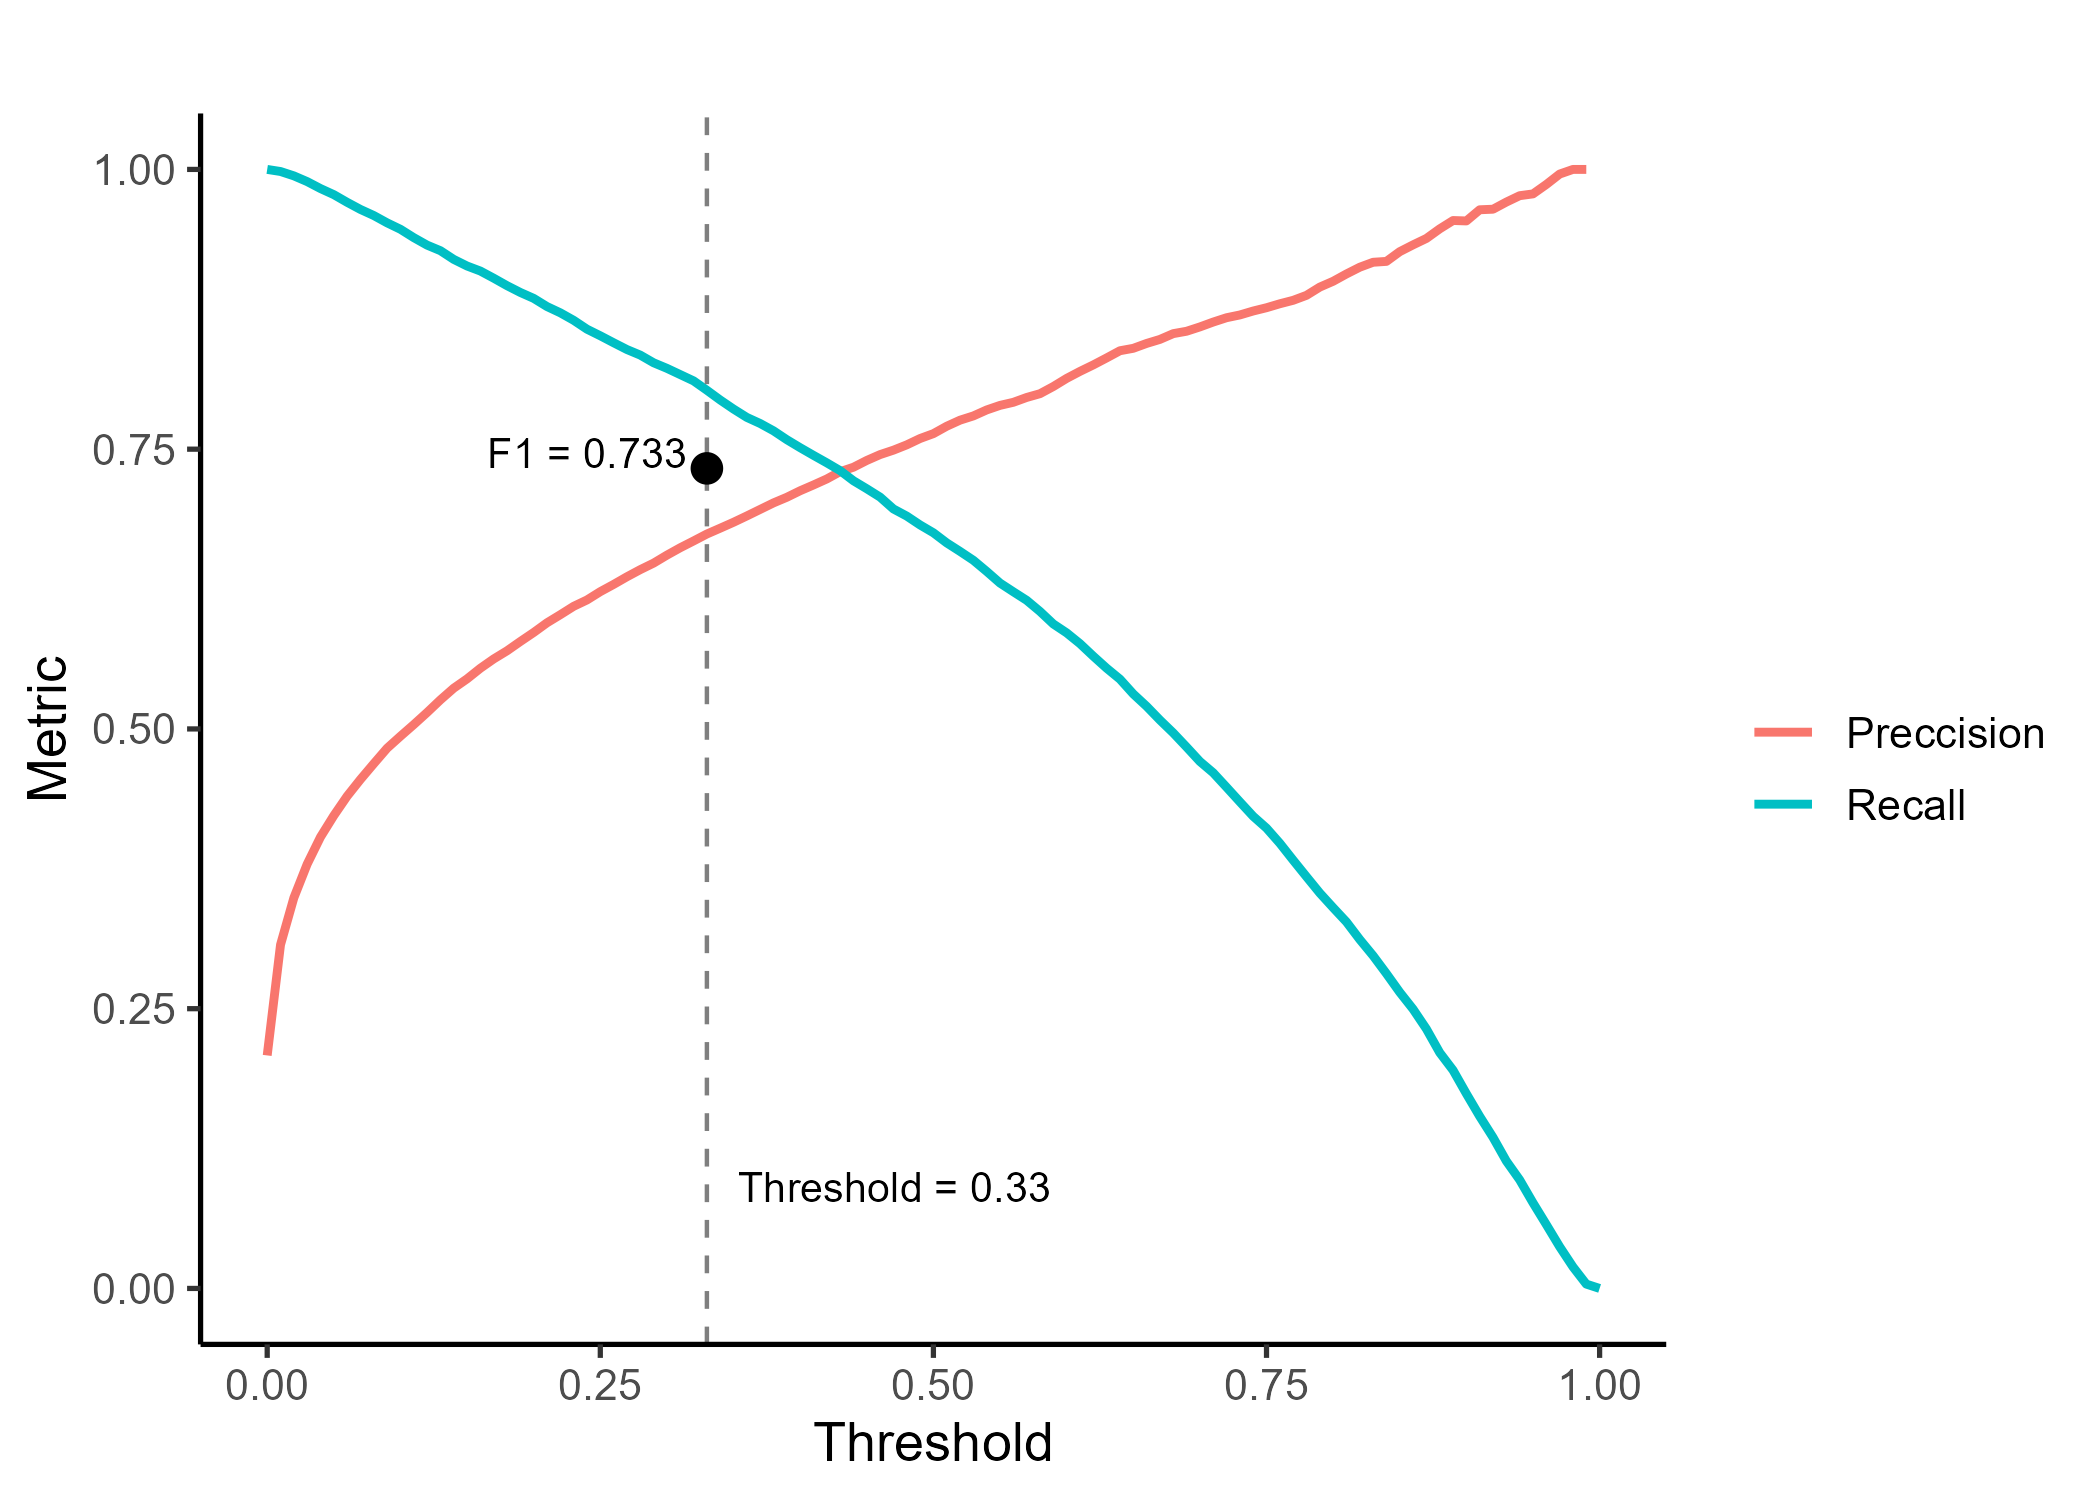
\includegraphics[width=0.5\textwidth]{visuals/3_1_metricas/02_pr_values.png} 
\end{figure}

A pesar de la tolerancia y el desbalance presente en los datos, la optimización del modelo permite mantener un equilibrio adecuado entre precisión y recall, con valores de 0.81 y 0.80 para la clase \textit{Pobre (Sí)}, y de 0.90 y 0.91 para la clase \textit{Pobre (No)}, respectivamente. En ambos casos, el F1-score se mantiene cercano a 0.80 y 0.90, lo que muestra que el modelo conserva un buen nivel de desempeño tanto en la identificación de hogares pobres como en la clasificación correcta de los no pobres. Asimismo, se observa en la Tabla \ref{tab:confusion_best_model}, la matriz de confusión respalda estos resultados al mostrar una alta proporción de observaciones correctamente clasificadas en la diagonal.

\begin{table}[H]
\centering
\caption{Matriz de confusión del modelo}
\input{visuals/3_1_metricas/03_tabla_confuson_estandarizada.txt}
\label{tab:confusion_best_model}
\end{table}

Finalmente, los modelos de XGBoost mostraron el mejor desempeño general. Tanto la versión ponderada como la no ponderada superaron el F1 de 0.70. En particular, el modelo con pesos alcanzó un Recall de 0.832, destacándose por su capacidad para identificar correctamente a los hogares pobres. Sin embargo, al ajustar el punto de corte según la métrica F1, como se muestra en la Tabla 2, el modelo sin pesos logró un rendimiento ligeramente superior en el conjunto de prueba. Aunque su Precision fue 0.12 puntos inferior, su Recall más alto compensó esta diferencia, permitiéndole alcanzar un F1 final superior. En consecuencia, el modelo XGBoost sin pesos se consolidó como la mejor alternativa para la predicción de pobreza, combinando eficacia, parsimonia y estabilidad en sus resultados.







%-------------------------------------------------%
%-------------------------------------------------%
%-------------------------------------------------%

%-------------------------------------------------%
%-------------------------------------------------%
%-------------------------------------------------%

\subsection{Kaggle - Competencia}

La comparación entre las seis configuraciones con mejor desempeño de la competencia que corresponden al algoritmo de XGBoost muestra que las diferencias marginales en el puntaje F1 (entre 70 y 73) se explican principalmente por variaciones en el ajuste de hiperparámetros y en las estrategias de ponderación, más que por cambios estructurales en el modelo. El modelo con mayor rendimiento (F1 = 73) utilizó una tasa de aprendizaje moderada ($\eta = 0.04$), una profundidad intermedia (7) y un valor alto de min\_child\_weight (25), combinación que favoreció la capacidad de generalización y mitigó el sobreajuste. En contraste, las configuraciones con mayor profundidad (8--10) o tasas de aprendizaje más bajas mostraron ligeras caídas de desempeño, lo que induce a creer que una mayor complejidad llevó a capturar ruido idiosincrático de las clases minoritarias. Ver tabla \ref{tab:comparacion_xgb}

Cabe destacar que la inclusión de ponderaciones por instancia mejoró la estabilidad del rendimiento en varias especificaciones, especialmente cuando se combinaron con valores elevados de colsample\_bytree (0.8--0.9) y subsample (0.9--1). Sin embargo, un muestreo excesivo de características generó leves fluctuaciones entre pliegues de validación, lo que explica la meseta observada entre F1 = 71 y 72. El hecho de que el mejor modelo no implementara re-balanceo, pero sí optimizara directamente sobre la métrica F1, resultó eficaz, lo que indica que la distribución original de los datos fue capturada adecuadamente mediante la regularización y no requirió ajuste explícito de frecuencias.

En conjunto, la superioridad del modelo líder no se debe a una diferencia estructural, sino a una estrategia de optimización: una tasa de aprendizaje controlada, profundidad limitada y muestreo conservador, que lograron maximizar la sensibilidad sin aumentar los falsos positivos. La estabilidad del puntaje F1 entre las configuraciones más competitivas muestra que, a partir de cierto umbral de desempeño, las ganancias adicionales en \texttt{XGBoost} dependen menos de la arquitectura del modelo y más de la calibración fina de los parámetros de regularización y de la dinámica de aprendizaje.




\begin{table}[H]
\centering
\caption{Comparación de modelos XGBoost}
\label{tab:comparacion_xgb}
\resizebox{\textwidth}{!}{%
\begin{tabular}{@{}cccccccccccc@{}}
\toprule
\textbf{Top} & 
\textbf{Algoritmo} & 
\textbf{Métrica} & 
\textbf{Rebalanceo} & 
\textbf{Trees} & 
\textbf{Eta} & 
\makecell{\textbf{max}\\\textbf{depth}} & 
\makecell{\textbf{min\_child}\\\textbf{weight}} & 
\textbf{Gamma} & 
\makecell{\textbf{colsample}\\\textbf{bytree}} & 
\textbf{subsample} & 
\textbf{F1-Score} \\ 
\midrule
1 & XGBoost & F1 & No & 500 & 0.04 & 7 & 25 & 0 & 0.6 & 0.8 & 73 \\
2 & XGBoost & F1 & Weights & 500 & 0.03 & 8 & 25 & 0 & 0.8 & 0.9 & 72 \\
3 & XGBoost & F1 & Weights & 500 & 0.05 & 10 & 20 & 1 & 0.9 & 1 & 72 \\
4 & XGBoost & Regla de Bayes & Weights & 500 & 0.03 & 8 & 25 & 0 & 0.8 & 0.9 & 72 \\
5 & XGBoost & Regla de Bayes & No & 500 & 0.03 & 8 & 25 & 0 & 0.8 & 0.9 & 71 \\
6 & XGBoost & Regla de Bayes & No & 500 & 0.04 & 7 & 25 & 0 & 0.6 & 0.8 & 70 \\
\bottomrule
\end{tabular}%
}
\end{table}
\medskip
\begin{minipage}{\textwidth}
\tiny
\textit{Nota:}  Esta tabla muestra,las seis mejores predicciones de la competencia en Kaggle.

\end{minipage}

\subsection{Importancia de variables}

En esta sección se presenta la importancia relativa de las variables del modelo con mejor desempeño según el F1-score. La estimación se realiza mediante el método de \textit{importancia por permutación}, que mide la pérdida en el \textit{F1} al alterar aleatoriamente los valores de una variable \( X_j \), manteniendo las demás constantes. Formalmente:

\begin{equation}
VI_j = \text{F1}(X) - \text{F1}(X_{-j}, \pi(X_j))
\label{eq:vi}
\end{equation}

donde \( \pi(X_j) \) es una permutación aleatoria de \( X_j \). Un mayor \( VI_j \) indica una variable más influyente en las predicciones del modelo.


La Figura \ref{fig:vipgen} muestra cómo se distribuye la importancia acumulada por categoría de variables, lo cual permite identificar qué grupos contribuyen en mayor medida a la capacidad predictiva del modelo. En particular, las características del hogar concentran el 48,9\% de la importancia total, seguidas de las características de los miembros  del hogar (40,61\%), y los ocupados del hogar (10,4\%). Estos resultados apuntan a que las condiciones del hogar y sus miembros son factores principales para predecir la probabilidad de pobreza.

\begin{figure}[H] 
    \centering
    \caption{VI - Categoría}
    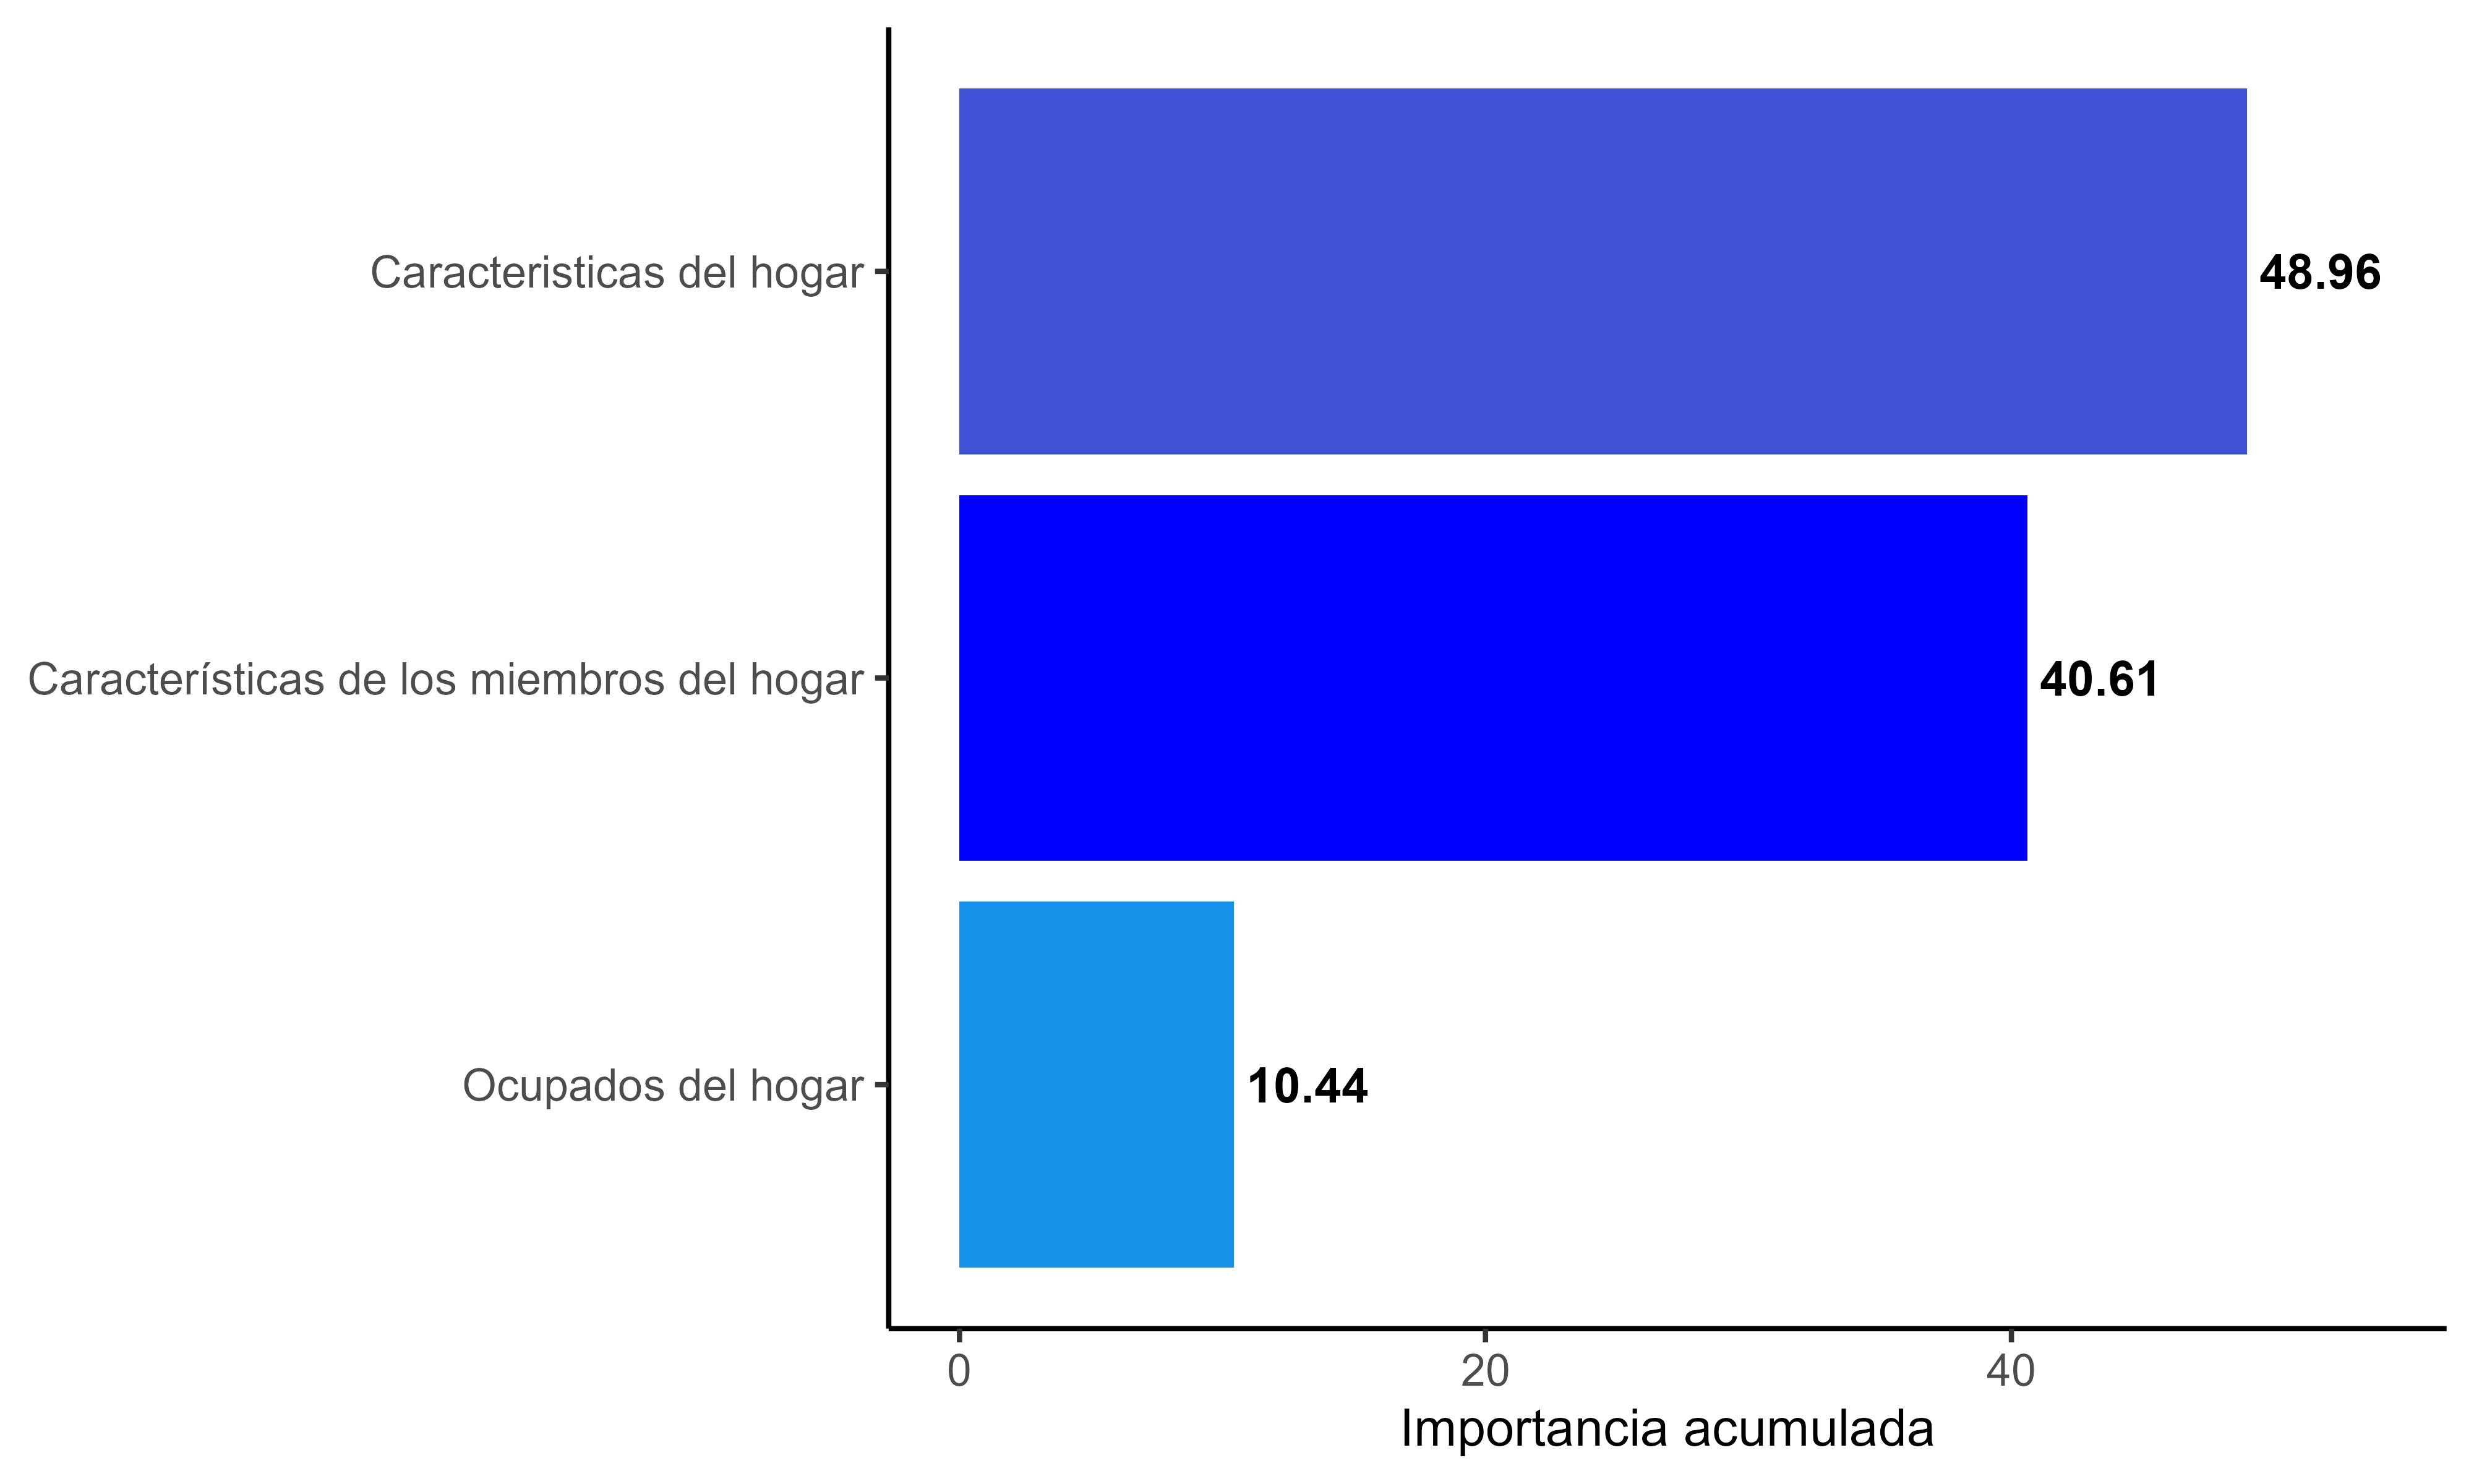
\includegraphics[width=0.7\linewidth]{visuals/02_vip_gen.png}
    \label{fig:vipgen}\\
 \vspace{0.3em}
\end{figure}

De forma complementaria, la Figura \ref{fig:vip10} presenta las diez variables con mayor importancia relativa. Sobresalen el valor del arriendo, el número de personas afiliadas al régimen contributivo y el  número de ocupados promedio, que en conjunto explican más del 50\% de la capacidad predictiva total. Estas variables representan aspectos clave del bienestar del hogar, como la inserción laboral, las condiciones habitacionales y el acceso a la protección social. 

Adicionalmente, se reentrenó el modelo \textit{XGBoost} empleando únicamente estas diez variables. Mientras el modelo completo alcanzó un \textit{F1-score} del 73\%, la versión reducida obtuvo un 69.6\%, lo que demuestra que una fracción acotada de predictores concentra buena parte del poder explicativo del modelo. Este hallazgo evidencia que es posible predecir la pobreza con un nivel de precisión aceptable utilizando un conjunto reducido de indicadores, destacando la solidez de las variables más relevantes y su potencial para aplicaciones en contextos con información limitada.
\begin{figure}[H] 
    \centering
    \caption{VI - Top 10}
    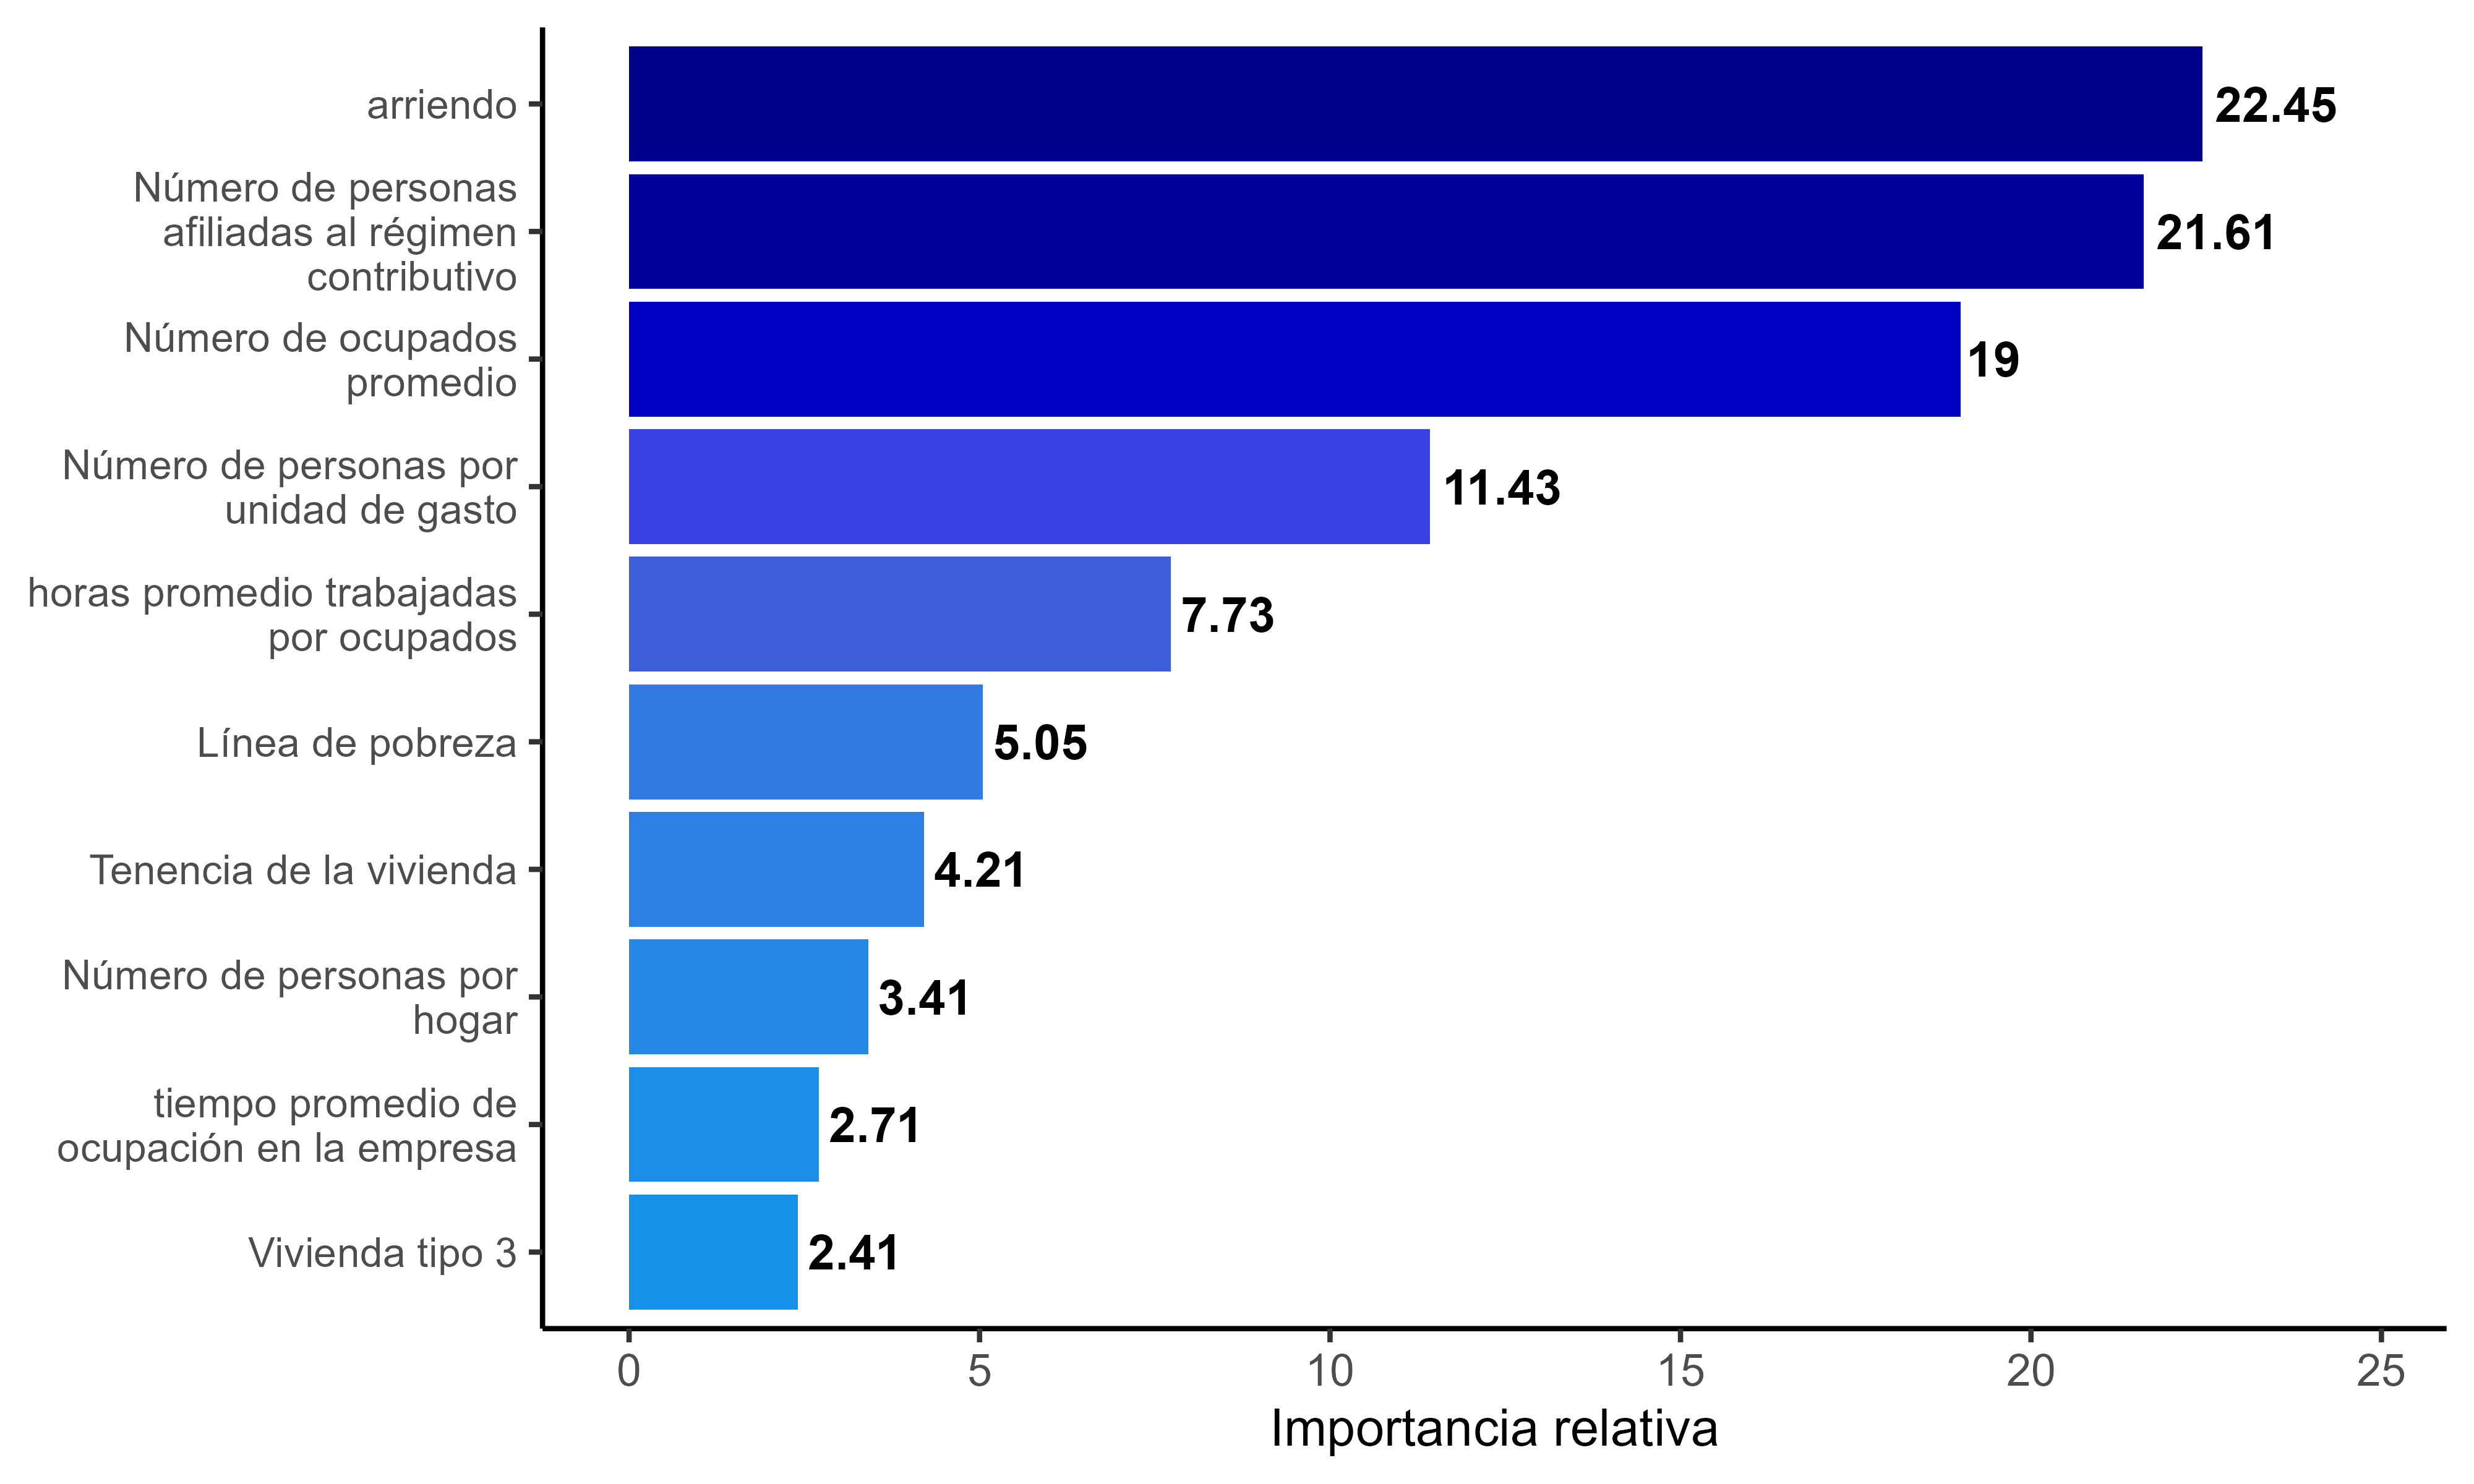
\includegraphics[width=0.8\linewidth]{visuals/02_vip_10.png}
    \label{fig:vip10}\\
 \vspace{0.3em}
\end{figure}